\documentclass{standalone}
\usepackage{tikz}
\usetikzlibrary{calc,arrows.meta,decorations.markings,math,patterns}
\ifpdftex\usepackage[scaled=1]{helvet}\fi
\ifxetex\usepackage{fontspec}\setsansfont{TeX Gyre Heros}\fi
\begin{document}
\begingroup
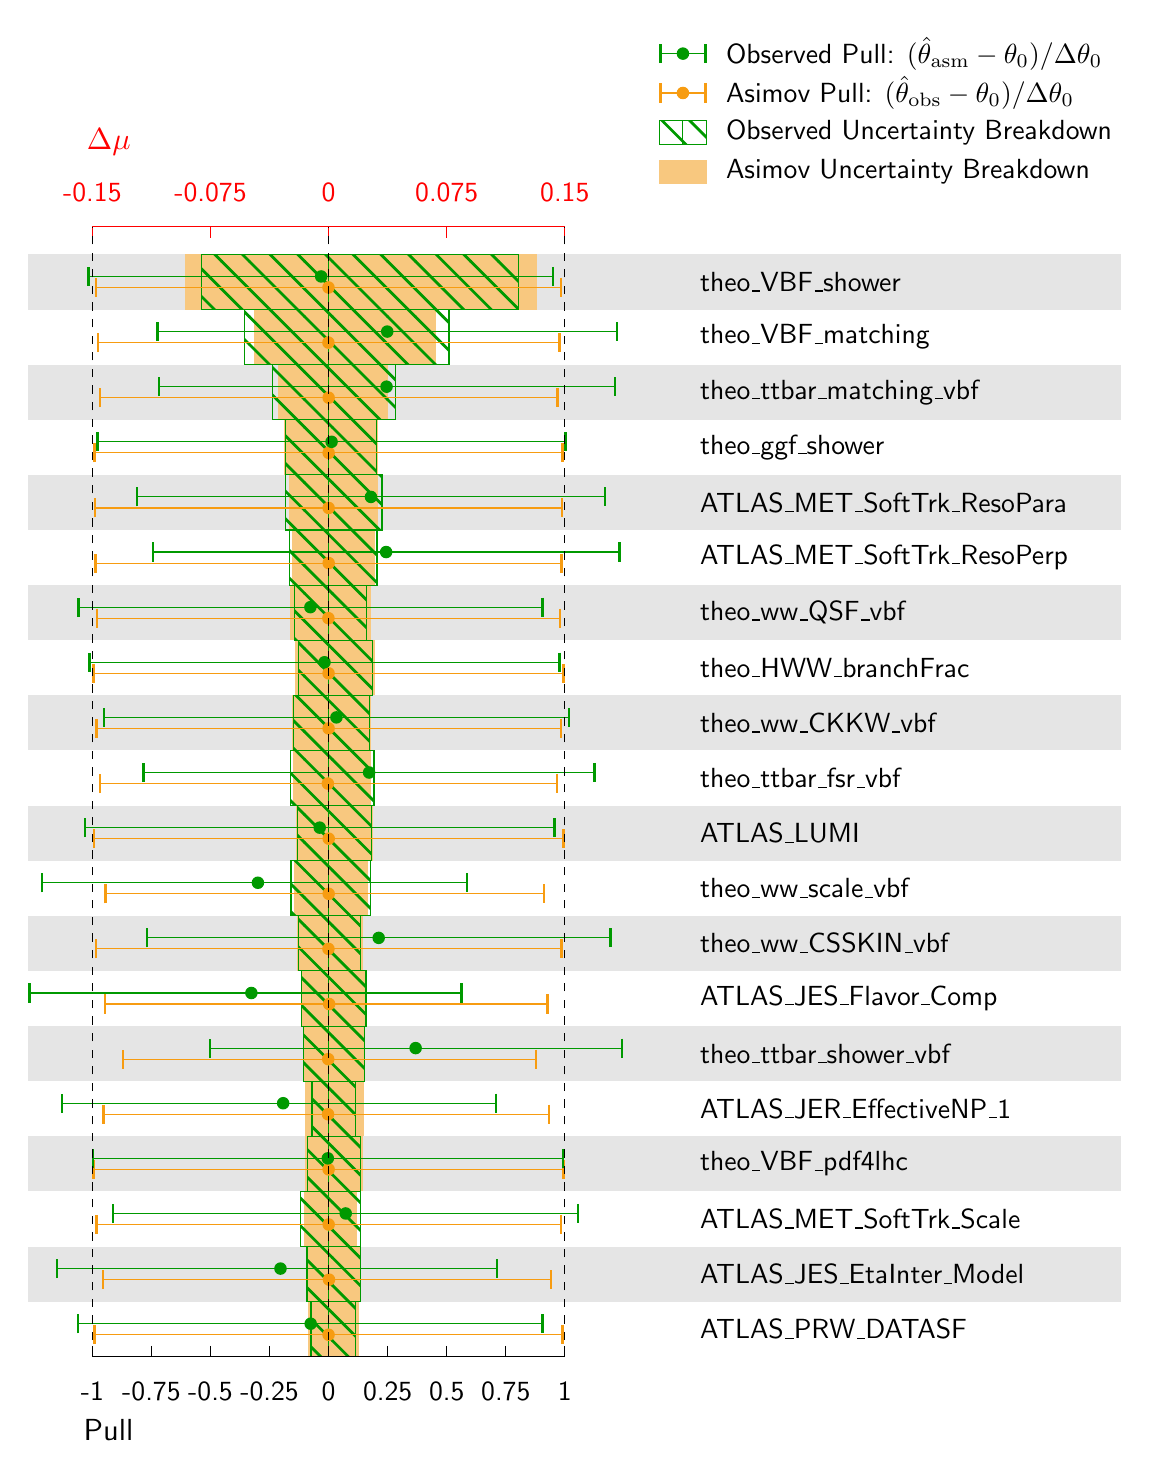
\begin{tikzpicture}[x=3cm,y=.7cm,%
  axlbl/.style={scale=1,anchor=center},%
  pull/.style={{|[scale=1.5, line width=0.3mm]}-{|[scale=1.5, line width=0.3mm]}},%scale is error vertical bar size
  dot/.style={circle,fill,inner sep=1pt,scale=1.6},
  every node/.append style={line width=2mm,font=\sffamily}
]

  % defining the new dimensions and parameters
\newlength{\hatchspread}
\newlength{\hatchthickness}
\newlength{\hatchshift}
\newcommand{\hatchcolor}{}
% declaring the keys in tikz
\tikzset{hatchspread/.code={\setlength{\hatchspread}{#1}},
         hatchthickness/.code={\setlength{\hatchthickness}{#1}},
         hatchshift/.code={\setlength{\hatchshift}{#1}},% must be >= 0
         hatchcolor/.code={\renewcommand{\hatchcolor}{#1}}}
% setting the default values
\tikzset{hatchspread=1pt,
         hatchthickness=1pt,
         hatchshift=0pt,% must be >= 0
         hatchcolor=black}
% declaring the pattern
\pgfdeclarepatternformonly[\hatchspread,\hatchthickness,\hatchshift,\hatchcolor]% variables
   {custom north west lines}% name
   {\pgfqpoint{\dimexpr-2\hatchthickness}{\dimexpr-2\hatchthickness}}% lower left corner
   {\pgfqpoint{\dimexpr\hatchspread+2\hatchthickness}{\dimexpr\hatchspread+2\hatchthickness}}% upper right corner
   {\pgfqpoint{\dimexpr\hatchspread}{\dimexpr\hatchspread}}% tile size
   {% shape description
    \pgfsetlinewidth{\hatchthickness}
    \pgfpathmoveto{\pgfqpoint{0pt}{\dimexpr\hatchspread+\hatchshift}}
    \pgfpathlineto{\pgfqpoint{\dimexpr\hatchspread+0.15pt+\hatchshift}{-0.15pt}}
    \ifdim \hatchshift > 0pt
      \pgfpathmoveto{\pgfqpoint{0pt}{\hatchshift}}
      \pgfpathlineto{\pgfqpoint{\dimexpr0.15pt+\hatchshift}{-0.15pt}}
    \fi
    \pgfsetstrokecolor{\hatchcolor}
    \pgfusepath{stroke}
   }
  
\definecolor{colOverlay.Ranking.BREAKDOWNS.observedTwoPos}{rgb}{0.972549,0.784314,0.498039}
\definecolor{colOverlay.Ranking.BREAKDOWNS.observedTwoNeg}{rgb}{0.972549,0.784314,0.498039}
\definecolor{colOverlay.Ranking.BREAKDOWNS.observedTwoHatchPos}{rgb}{0.972549,0.784314,0.498039}
\definecolor{colOverlay.Ranking.BREAKDOWNS.observedTwoHatchNeg}{rgb}{0.972549,0.784314,0.498039}
\tikzset{Overlay.Ranking.BREAKDOWNS.observedTwoPos/.style={draw=none,fill=colOverlay.Ranking.BREAKDOWNS.observedTwoPos,text opacity = 1.0, fill opacity=1,}}
\tikzset{Overlay.Ranking.BREAKDOWNS.observedTwoNeg/.style={draw=none,fill=colOverlay.Ranking.BREAKDOWNS.observedTwoNeg,text opacity = 1.0, fill opacity=1,}}
\definecolor{colOverlay.Ranking.BREAKDOWNS.observedPos}{rgb}{0.000000,0.600000,0.000000}
\definecolor{colOverlay.Ranking.BREAKDOWNS.observedNeg}{rgb}{0.000000,0.600000,0.000000}
\definecolor{colOverlay.Ranking.BREAKDOWNS.observedHatchPos}{rgb}{0.000000,0.600000,0.000000}
\definecolor{colOverlay.Ranking.BREAKDOWNS.observedHatchNeg}{rgb}{0.000000,0.600000,0.000000}
\tikzset{Overlay.Ranking.BREAKDOWNS.observedPos/.style={draw=colOverlay.Ranking.BREAKDOWNS.observedPos,pattern=custom north west lines, hatchcolor=colOverlay.Ranking.BREAKDOWNS.observedHatchPos,hatchspread=10pt,}}
\tikzset{Overlay.Ranking.BREAKDOWNS.observedNeg/.style={draw=colOverlay.Ranking.BREAKDOWNS.observedNeg,pattern=custom north west lines, hatchcolor=colOverlay.Ranking.BREAKDOWNS.observedHatchNeg,hatchspread=10pt,}}
\definecolor{colEffectAxes}{rgb}{1.000000,0.000000,0.000000}
\definecolor{colOverlay.Pulls.PULLS.observedTwo}{rgb}{0.968627,0.611765,0.066667}
\tikzset{Overlay.Pulls.PULLS.observedTwo/.style={pull,color=colOverlay.Pulls.PULLS.observedTwo}}
\definecolor{colOverlay.Pulls.PULLS.observed}{rgb}{0.000000,0.600000,0.000000}
\tikzset{Overlay.Pulls.PULLS.observed/.style={pull,color=colOverlay.Pulls.PULLS.observed}}
\definecolor{colPullAxes}{rgb}{0.000000,0.000000,0.000000}
\definecolor{colHighlighting}{rgb}{0.900000,0.900000,0.900000}
\begin{scope}[name=legend,shift={(1.5,1)},x=0.3cm,y=.5cm]\draw[Overlay.Ranking.BREAKDOWNS.observedTwoNeg](-1,-0.3) rectangle (0,0.3);
\draw[Overlay.Ranking.BREAKDOWNS.observedTwoPos](0,-0.3) rectangle (1,0.3);
\node[anchor=west] at(1.1,0){Asimov Uncertainty Breakdown};
\draw[Overlay.Ranking.BREAKDOWNS.observedNeg](-1,0.7) rectangle (0,1.3);
\draw[Overlay.Ranking.BREAKDOWNS.observedPos](0,0.7) rectangle (1,1.3);
\node[anchor=west] at(1.1,1){Observed Uncertainty Breakdown};
\draw[Overlay.Pulls.PULLS.observedTwo](-1,2) -- (1,2);\node[dot,colOverlay.Pulls.PULLS.observedTwo] at (0,2) {};
\node[anchor=west] at(1.1,2){Asimov Pull: $(\hat{\theta}_{\mathrm{obs}} - \theta_0) / \Delta \theta_0$};
\draw[Overlay.Pulls.PULLS.observed](-1,3) -- (1,3);\node[dot,colOverlay.Pulls.PULLS.observed] at (0,3) {};
\node[anchor=west] at(1.1,3){Observed Pull: $(\hat{\theta}_{\mathrm{asm}} - \theta_0) / \Delta \theta_0$};
\end{scope}\pgfdeclarelayer{background}\pgfsetlayers{background,main}
\node[scale=1,anchor=west,rotate=0] at (1.5,-1) {theo\_VBF\_shower};
\node[scale=1,anchor=west,rotate=0] at (1.5,-2) {theo\_VBF\_matching};
\node[scale=1,anchor=west,rotate=0] at (1.5,-3) {theo\_ttbar\_matching\_vbf};
\node[scale=1,anchor=west,rotate=0] at (1.5,-4) {theo\_ggf\_shower};
\node[scale=1,anchor=west,rotate=0] at (1.5,-5) {ATLAS\_MET\_SoftTrk\_ResoPara};
\node[scale=1,anchor=west,rotate=0] at (1.5,-6) {ATLAS\_MET\_SoftTrk\_ResoPerp};
\node[scale=1,anchor=west,rotate=0] at (1.5,-7) {theo\_ww\_QSF\_vbf};
\node[scale=1,anchor=west,rotate=0] at (1.5,-8) {theo\_HWW\_branchFrac};
\node[scale=1,anchor=west,rotate=0] at (1.5,-9) {theo\_ww\_CKKW\_vbf};
\node[scale=1,anchor=west,rotate=0] at (1.5,-10) {theo\_ttbar\_fsr\_vbf};
\node[scale=1,anchor=west,rotate=0] at (1.5,-11) {ATLAS\_LUMI};
\node[scale=1,anchor=west,rotate=0] at (1.5,-12) {theo\_ww\_scale\_vbf};
\node[scale=1,anchor=west,rotate=0] at (1.5,-13) {theo\_ww\_CSSKIN\_vbf};
\node[scale=1,anchor=west,rotate=0] at (1.5,-14) {ATLAS\_JES\_Flavor\_Comp};
\node[scale=1,anchor=west,rotate=0] at (1.5,-15) {theo\_ttbar\_shower\_vbf};
\node[scale=1,anchor=west,rotate=0] at (1.5,-16) {ATLAS\_JER\_EffectiveNP\_1};
\node[scale=1,anchor=west,rotate=0] at (1.5,-17) {theo\_VBF\_pdf4lhc};
\node[scale=1,anchor=west,rotate=0] at (1.5,-18) {ATLAS\_MET\_SoftTrk\_Scale};
\node[scale=1,anchor=west,rotate=0] at (1.5,-19) {ATLAS\_JES\_EtaInter\_Model};
\node[scale=1,anchor=west,rotate=0] at (1.5,-20) {ATLAS\_PRW\_DATASF};
\begin{scope}[name=ranking,colEffectAxes,xscale=6.66667]
  \draw[Overlay.Ranking.BREAKDOWNS.observedTwoNeg](-0.091074,-1.5) rectangle (0,-0.5);
  \draw[Overlay.Ranking.BREAKDOWNS.observedTwoPos](0,-1.5) rectangle (0.132236,-0.5);
  \draw[Overlay.Ranking.BREAKDOWNS.observedTwoNeg](-0.0470736,-2.5) rectangle (0,-1.5);
  \draw[Overlay.Ranking.BREAKDOWNS.observedTwoPos](0,-2.5) rectangle (0.0679128,-1.5);
  \draw[Overlay.Ranking.BREAKDOWNS.observedTwoNeg](-0.0320696,-3.5) rectangle (0,-2.5);
  \draw[Overlay.Ranking.BREAKDOWNS.observedTwoPos](0,-3.5) rectangle (0.0376506,-2.5);
  \draw[Overlay.Ranking.BREAKDOWNS.observedTwoNeg](-0.0282914,-4.5) rectangle (0,-3.5);
  \draw[Overlay.Ranking.BREAKDOWNS.observedTwoPos](0,-4.5) rectangle (0.0312566,-3.5);
  \draw[Overlay.Ranking.BREAKDOWNS.observedTwoNeg](-0.024838,-5.5) rectangle (0,-4.5);
  \draw[Overlay.Ranking.BREAKDOWNS.observedTwoPos](0,-5.5) rectangle (0.0313573,-4.5);
  \draw[Overlay.Ranking.BREAKDOWNS.observedTwoNeg](-0.0232541,-6.5) rectangle (0,-5.5);
  \draw[Overlay.Ranking.BREAKDOWNS.observedTwoPos](0,-6.5) rectangle (0.0292411,-5.5);
  \draw[Overlay.Ranking.BREAKDOWNS.observedTwoNeg](-0.0242062,-7.5) rectangle (0,-6.5);
  \draw[Overlay.Ranking.BREAKDOWNS.observedTwoPos](0,-7.5) rectangle (0.0270654,-6.5);
  \draw[Overlay.Ranking.BREAKDOWNS.observedTwoNeg](-0.0211147,-8.5) rectangle (0,-7.5);
  \draw[Overlay.Ranking.BREAKDOWNS.observedTwoPos](0,-8.5) rectangle (0.0296135,-7.5);
  \draw[Overlay.Ranking.BREAKDOWNS.observedTwoNeg](-0.0232354,-9.5) rectangle (0,-8.5);
  \draw[Overlay.Ranking.BREAKDOWNS.observedTwoPos](0,-9.5) rectangle (0.0272164,-8.5);
  \draw[Overlay.Ranking.BREAKDOWNS.observedTwoNeg](-0.0223754,-10.5) rectangle (0,-9.5);
  \draw[Overlay.Ranking.BREAKDOWNS.observedTwoPos](0,-10.5) rectangle (0.0269073,-9.5);
  \draw[Overlay.Ranking.BREAKDOWNS.observedTwoNeg](-0.0209003,-11.5) rectangle (0,-10.5);
  \draw[Overlay.Ranking.BREAKDOWNS.observedTwoPos](0,-11.5) rectangle (0.0281354,-10.5);
  \draw[Overlay.Ranking.BREAKDOWNS.observedTwoNeg](-0.0222123,-12.5) rectangle (0,-11.5);
  \draw[Overlay.Ranking.BREAKDOWNS.observedTwoPos](0,-12.5) rectangle (0.024944,-11.5);
  \draw[Overlay.Ranking.BREAKDOWNS.observedTwoNeg](-0.0201193,-13.5) rectangle (0,-12.5);
  \draw[Overlay.Ranking.BREAKDOWNS.observedTwoPos](0,-13.5) rectangle (0.0216954,-12.5);
  \draw[Overlay.Ranking.BREAKDOWNS.observedTwoNeg](-0.0169072,-14.5) rectangle (0,-13.5);
  \draw[Overlay.Ranking.BREAKDOWNS.observedTwoPos](0,-14.5) rectangle (0.0233872,-13.5);
  \draw[Overlay.Ranking.BREAKDOWNS.observedTwoNeg](-0.0154971,-15.5) rectangle (0,-14.5);
  \draw[Overlay.Ranking.BREAKDOWNS.observedTwoPos](0,-15.5) rectangle (0.0223058,-14.5);
  \draw[Overlay.Ranking.BREAKDOWNS.observedTwoNeg](-0.0151889,-16.5) rectangle (0,-15.5);
  \draw[Overlay.Ranking.BREAKDOWNS.observedTwoPos](0,-16.5) rectangle (0.0223573,-15.5);
  \draw[Overlay.Ranking.BREAKDOWNS.observedTwoNeg](-0.0149257,-17.5) rectangle (0,-16.5);
  \draw[Overlay.Ranking.BREAKDOWNS.observedTwoPos](0,-17.5) rectangle (0.0217462,-16.5);
  \draw[Overlay.Ranking.BREAKDOWNS.observedTwoNeg](-0.0155778,-18.5) rectangle (0,-17.5);
  \draw[Overlay.Ranking.BREAKDOWNS.observedTwoPos](0,-18.5) rectangle (0.0178573,-17.5);
  \draw[Overlay.Ranking.BREAKDOWNS.observedTwoNeg](-0.0132977,-19.5) rectangle (0,-18.5);
  \draw[Overlay.Ranking.BREAKDOWNS.observedTwoPos](0,-19.5) rectangle (0.0200937,-18.5);
  \draw[Overlay.Ranking.BREAKDOWNS.observedTwoNeg](-0.0132822,-20.5) rectangle (0,-19.5);
  \draw[Overlay.Ranking.BREAKDOWNS.observedTwoPos](0,-20.5) rectangle (0.019305,-19.5);
  \draw[Overlay.Ranking.BREAKDOWNS.observedNeg](-0.0805606,-1.5) rectangle (0,-0.5);
  \draw[Overlay.Ranking.BREAKDOWNS.observedPos](0,-1.5) rectangle (0.120544,-0.5);
  \draw[Overlay.Ranking.BREAKDOWNS.observedNeg](-0.0531906,-2.5) rectangle (0,-1.5);
  \draw[Overlay.Ranking.BREAKDOWNS.observedPos](0,-2.5) rectangle (0.0764341,-1.5);
  \draw[Overlay.Ranking.BREAKDOWNS.observedNeg](-0.0357867,-3.5) rectangle (0,-2.5);
  \draw[Overlay.Ranking.BREAKDOWNS.observedPos](0,-3.5) rectangle (0.042283,-2.5);
  \draw[Overlay.Ranking.BREAKDOWNS.observedNeg](-0.027549,-4.5) rectangle (0,-3.5);
  \draw[Overlay.Ranking.BREAKDOWNS.observedPos](0,-4.5) rectangle (0.0302957,-3.5);
  \draw[Overlay.Ranking.BREAKDOWNS.observedNeg](-0.0271009,-5.5) rectangle (0,-4.5);
  \draw[Overlay.Ranking.BREAKDOWNS.observedPos](0,-5.5) rectangle (0.0339361,-4.5);
  \draw[Overlay.Ranking.BREAKDOWNS.observedNeg](-0.0246374,-6.5) rectangle (0,-5.5);
  \draw[Overlay.Ranking.BREAKDOWNS.observedPos](0,-6.5) rectangle (0.030713,-5.5);
  \draw[Overlay.Ranking.BREAKDOWNS.observedNeg](-0.0216573,-7.5) rectangle (0,-6.5);
  \draw[Overlay.Ranking.BREAKDOWNS.observedPos](0,-7.5) rectangle (0.0239078,-6.5);
  \draw[Overlay.Ranking.BREAKDOWNS.observedNeg](-0.0193882,-8.5) rectangle (0,-7.5);
  \draw[Overlay.Ranking.BREAKDOWNS.observedPos](0,-8.5) rectangle (0.027773,-7.5);
  \draw[Overlay.Ranking.BREAKDOWNS.observedNeg](-0.0225366,-9.5) rectangle (0,-8.5);
  \draw[Overlay.Ranking.BREAKDOWNS.observedPos](0,-9.5) rectangle (0.0262013,-8.5);
  \draw[Overlay.Ranking.BREAKDOWNS.observedNeg](-0.0242829,-10.5) rectangle (0,-9.5);
  \draw[Overlay.Ranking.BREAKDOWNS.observedPos](0,-10.5) rectangle (0.0288228,-9.5);
  \draw[Overlay.Ranking.BREAKDOWNS.observedNeg](-0.0198752,-11.5) rectangle (0,-10.5);
  \draw[Overlay.Ranking.BREAKDOWNS.observedPos](0,-11.5) rectangle (0.0270856,-10.5);
  \draw[Overlay.Ranking.BREAKDOWNS.observedNeg](-0.0238566,-12.5) rectangle (0,-11.5);
  \draw[Overlay.Ranking.BREAKDOWNS.observedPos](0,-12.5) rectangle (0.0268139,-11.5);
  \draw[Overlay.Ranking.BREAKDOWNS.observedNeg](-0.0190373,-13.5) rectangle (0,-12.5);
  \draw[Overlay.Ranking.BREAKDOWNS.observedPos](0,-13.5) rectangle (0.0204718,-12.5);
  \draw[Overlay.Ranking.BREAKDOWNS.observedNeg](-0.0172235,-14.5) rectangle (0,-13.5);
  \draw[Overlay.Ranking.BREAKDOWNS.observedPos](0,-14.5) rectangle (0.0237604,-13.5);
  \draw[Overlay.Ranking.BREAKDOWNS.observedNeg](-0.0161185,-15.5) rectangle (0,-14.5);
  \draw[Overlay.Ranking.BREAKDOWNS.observedPos](0,-15.5) rectangle (0.02268,-14.5);
  \draw[Overlay.Ranking.BREAKDOWNS.observedNeg](-0.0105187,-16.5) rectangle (0,-15.5);
  \draw[Overlay.Ranking.BREAKDOWNS.observedPos](0,-16.5) rectangle (0.0168417,-15.5);
  \draw[Overlay.Ranking.BREAKDOWNS.observedNeg](-0.0135741,-17.5) rectangle (0,-16.5);
  \draw[Overlay.Ranking.BREAKDOWNS.observedPos](0,-17.5) rectangle (0.0203311,-16.5);
  \draw[Overlay.Ranking.BREAKDOWNS.observedNeg](-0.0178362,-18.5) rectangle (0,-17.5);
  \draw[Overlay.Ranking.BREAKDOWNS.observedPos](0,-18.5) rectangle (0.0203331,-17.5);
  \draw[Overlay.Ranking.BREAKDOWNS.observedNeg](-0.0137088,-19.5) rectangle (0,-18.5);
  \draw[Overlay.Ranking.BREAKDOWNS.observedPos](0,-19.5) rectangle (0.0202253,-18.5);
  \draw[Overlay.Ranking.BREAKDOWNS.observedNeg](-0.0111807,-20.5) rectangle (0,-19.5);
  \draw[Overlay.Ranking.BREAKDOWNS.observedPos](0,-20.5) rectangle (0.0167935,-19.5);
  \draw (0,-0.2) -- (0,0) node [axlbl,above=3pt]{0};
  \draw (0.075,-0.2) -- (0.075,0) node [axlbl,above=3pt]{0.075};
  \draw (0.15,-0.2) -- (0.15,0) node [axlbl,above=3pt]{0.15};
  \draw (-0.075,-0.2) -- (-0.075,0) node [axlbl,above=3pt]{-0.075};
  \draw (-0.15,-0.2) -- (-0.15,0) node [axlbl,above=3pt]{-0.15};
  \draw (-0.15,0) -- (0.15,0);
  \node[axlbl,above left=5pt,scale=1.1] at (-0.105,0.7) {$\Delta\mu$};
\end{scope}
\begin{scope}[name=pulls]
  \draw[Overlay.Pulls.PULLS.observedTwo] (-0.990492,-1.1) -- (0.987782,-1.1);  \node[dot,colOverlay.Pulls.PULLS.observedTwo] at (-0.000504648,-1.1) {};
  \draw[Overlay.Pulls.PULLS.observedTwo] (-0.979873,-2.1) -- (0.981765,-2.1);  \node[dot,colOverlay.Pulls.PULLS.observedTwo] at (-0.000874235,-2.1) {};
  \draw[Overlay.Pulls.PULLS.observedTwo] (-0.973069,-3.1) -- (0.974636,-3.1);  \node[dot,colOverlay.Pulls.PULLS.observedTwo] at (0.00022575,-3.1) {};
  \draw[Overlay.Pulls.PULLS.observedTwo] (-0.995998,-4.1) -- (0.995868,-4.1);  \node[dot,colOverlay.Pulls.PULLS.observedTwo] at (0.00020421,-4.1) {};
  \draw[Overlay.Pulls.PULLS.observedTwo] (-0.992743,-5.1) -- (0.992557,-5.1);  \node[dot,colOverlay.Pulls.PULLS.observedTwo] at (0.000231713,-5.1) {};
  \draw[Overlay.Pulls.PULLS.observedTwo] (-0.991345,-6.1) -- (0.991133,-6.1);  \node[dot,colOverlay.Pulls.PULLS.observedTwo] at (0.000336398,-6.1) {};
  \draw[Overlay.Pulls.PULLS.observedTwo] (-0.98622,-7.1) -- (0.984571,-7.1);  \node[dot,colOverlay.Pulls.PULLS.observedTwo] at (-0.000822051,-7.1) {};
  \draw[Overlay.Pulls.PULLS.observedTwo] (-0.999808,-8.1) -- (0.999809,-8.1);  \node[dot,colOverlay.Pulls.PULLS.observedTwo] at (-0.000144319,-8.1) {};
  \draw[Overlay.Pulls.PULLS.observedTwo] (-0.988237,-9.1) -- (0.988809,-9.1);  \node[dot,colOverlay.Pulls.PULLS.observedTwo] at (5.41663e-05,-9.1) {};
  \draw[Overlay.Pulls.PULLS.observedTwo] (-0.971931,-10.1) -- (0.971788,-10.1);  \node[dot,colOverlay.Pulls.PULLS.observedTwo] at (-0.00317065,-10.1) {};
  \draw[Overlay.Pulls.PULLS.observedTwo] (-0.998836,-11.1) -- (0.998845,-11.1);  \node[dot,colOverlay.Pulls.PULLS.observedTwo] at (0.000517744,-11.1) {};
  \draw[Overlay.Pulls.PULLS.observedTwo] (-0.948836,-12.1) -- (0.916643,-12.1);  \node[dot,colOverlay.Pulls.PULLS.observedTwo] at (0.000356133,-12.1) {};
  \draw[Overlay.Pulls.PULLS.observedTwo] (-0.990924,-13.1) -- (0.991601,-13.1);  \node[dot,colOverlay.Pulls.PULLS.observedTwo] at (-0.000622362,-13.1) {};
  \draw[Overlay.Pulls.PULLS.observedTwo] (-0.951623,-14.1) -- (0.931324,-14.1);  \node[dot,colOverlay.Pulls.PULLS.observedTwo] at (0.0023086,-14.1) {};
  \draw[Overlay.Pulls.PULLS.observedTwo] (-0.875213,-15.1) -- (0.882804,-15.1);  \node[dot,colOverlay.Pulls.PULLS.observedTwo] at (-0.00163655,-15.1) {};
  \draw[Overlay.Pulls.PULLS.observedTwo] (-0.957163,-16.1) -- (0.938327,-16.1);  \node[dot,colOverlay.Pulls.PULLS.observedTwo] at (-0.00234996,-16.1) {};
  \draw[Overlay.Pulls.PULLS.observedTwo] (-1.00002,-17.1) -- (1.00002,-17.1);  \node[dot,colOverlay.Pulls.PULLS.observedTwo] at (0.000136283,-17.1) {};
  \draw[Overlay.Pulls.PULLS.observedTwo] (-0.987904,-18.1) -- (0.987764,-18.1);  \node[dot,colOverlay.Pulls.PULLS.observedTwo] at (0.000264248,-18.1) {};
  \draw[Overlay.Pulls.PULLS.observedTwo] (-0.960823,-19.1) -- (0.946176,-19.1);  \node[dot,colOverlay.Pulls.PULLS.observedTwo] at (0.00173709,-19.1) {};
  \draw[Overlay.Pulls.PULLS.observedTwo] (-0.996032,-20.1) -- (0.994687,-20.1);  \node[dot,colOverlay.Pulls.PULLS.observedTwo] at (-0.000236391,-20.1) {};
  \draw[Overlay.Pulls.PULLS.observed] (-1.02108,-0.9) -- (0.955567,-0.9);  \node[dot,colOverlay.Pulls.PULLS.observed] at (-0.031488,-0.9) {};
  \draw[Overlay.Pulls.PULLS.observed] (-0.729095,-1.9) -- (1.22681,-1.9);  \node[dot,colOverlay.Pulls.PULLS.observed] at (0.248246,-1.9) {};
  \draw[Overlay.Pulls.PULLS.observed] (-0.723311,-2.9) -- (1.21744,-2.9);  \node[dot,colOverlay.Pulls.PULLS.observed] at (0.24537,-2.9) {};
  \draw[Overlay.Pulls.PULLS.observed] (-0.983539,-3.9) -- (1.00861,-3.9);  \node[dot,colOverlay.Pulls.PULLS.observed] at (0.0126076,-3.9) {};
  \draw[Overlay.Pulls.PULLS.observed] (-0.815919,-4.9) -- (1.17462,-4.9);  \node[dot,colOverlay.Pulls.PULLS.observed] at (0.17932,-4.9) {};
  \draw[Overlay.Pulls.PULLS.observed] (-0.748726,-5.9) -- (1.23603,-5.9);  \node[dot,colOverlay.Pulls.PULLS.observed] at (0.243508,-5.9) {};
  \draw[Overlay.Pulls.PULLS.observed] (-1.0645,-6.9) -- (0.910099,-6.9);  \node[dot,colOverlay.Pulls.PULLS.observed] at (-0.0770955,-6.9) {};
  \draw[Overlay.Pulls.PULLS.observed] (-1.01718,-7.9) -- (0.982434,-7.9);  \node[dot,colOverlay.Pulls.PULLS.observed] at (-0.0173818,-7.9) {};
  \draw[Overlay.Pulls.PULLS.observed] (-0.956507,-8.9) -- (1.0231,-8.9);  \node[dot,colOverlay.Pulls.PULLS.observed] at (0.0331354,-8.9) {};
  \draw[Overlay.Pulls.PULLS.observed] (-0.788015,-9.9) -- (1.13062,-9.9);  \node[dot,colOverlay.Pulls.PULLS.observed] at (0.171471,-9.9) {};
  \draw[Overlay.Pulls.PULLS.observed] (-1.03647,-10.9) -- (0.961122,-10.9);  \node[dot,colOverlay.Pulls.PULLS.observed] at (-0.0377192,-10.9) {};
  \draw[Overlay.Pulls.PULLS.observed] (-1.21845,-11.9) -- (0.589803,-11.9);  \node[dot,colOverlay.Pulls.PULLS.observed] at (-0.299234,-11.9) {};
  \draw[Overlay.Pulls.PULLS.observed] (-0.775076,-12.9) -- (1.19799,-12.9);  \node[dot,colOverlay.Pulls.PULLS.observed] at (0.21207,-12.9) {};
  \draw[Overlay.Pulls.PULLS.observed] (-1.27157,-13.9) -- (0.567448,-13.9);  \node[dot,colOverlay.Pulls.PULLS.observed] at (-0.326874,-13.9) {};
  \draw[Overlay.Pulls.PULLS.observed] (-0.50785,-14.9) -- (1.24752,-14.9);  \node[dot,colOverlay.Pulls.PULLS.observed] at (0.368403,-14.9) {};
  \draw[Overlay.Pulls.PULLS.observed] (-1.13372,-15.9) -- (0.714787,-15.9);  \node[dot,colOverlay.Pulls.PULLS.observed] at (-0.192394,-15.9) {};
  \draw[Overlay.Pulls.PULLS.observed] (-1.00327,-16.9) -- (0.996716,-16.9);  \node[dot,colOverlay.Pulls.PULLS.observed] at (-0.00327816,-16.9) {};
  \draw[Overlay.Pulls.PULLS.observed] (-0.91653,-17.9) -- (1.06087,-17.9);  \node[dot,colOverlay.Pulls.PULLS.observed] at (0.07244,-17.9) {};
  \draw[Overlay.Pulls.PULLS.observed] (-1.15587,-18.9) -- (0.718852,-18.9);  \node[dot,colOverlay.Pulls.PULLS.observed] at (-0.20372,-18.9) {};
  \draw[Overlay.Pulls.PULLS.observed] (-1.06651,-19.9) -- (0.910848,-19.9);  \node[dot,colOverlay.Pulls.PULLS.observed] at (-0.0758833,-19.9) {};
\draw[colPullAxes] (-1,-20.3) -- (-1,-20.5) node [axlbl,below=3pt]{-1};
\draw[colPullAxes] (-0.75,-20.3) -- (-0.75,-20.5) node [axlbl,below=3pt]{-0.75};
\draw[colPullAxes] (-0.5,-20.3) -- (-0.5,-20.5) node [axlbl,below=3pt]{-0.5};
\draw[colPullAxes] (-0.25,-20.3) -- (-0.25,-20.5) node [axlbl,below=3pt]{-0.25};
\draw[colPullAxes] (0,-20.3) -- (0,-20.5) node [axlbl,below=3pt]{0};
\draw[colPullAxes] (0.25,-20.3) -- (0.25,-20.5) node [axlbl,below=3pt]{0.25};
\draw[colPullAxes] (0.5,-20.3) -- (0.5,-20.5) node [axlbl,below=3pt]{0.5};
\draw[colPullAxes] (0.75,-20.3) -- (0.75,-20.5) node [axlbl,below=3pt]{0.75};
\draw[colPullAxes] (1,-20.3) -- (1,-20.5) node [axlbl,below=3pt]{1};
\node[axlbl,colPullAxes,anchor=north east,xshift=-1em,yshift=-1em,scale=1.1] at (-0.63,-20.8) {Pull};
\draw[colPullAxes] (-1,-20.5) -- (1,-20.5);
\draw[dashed,black] (0,-20.5) -- (0,0);
\draw[dashed,colPullAxes]   (-1,-20.5) -- (-1,0);
\draw[dashed,colPullAxes]   (1,-20.5) -- (1,0);
\end{scope}
\begin{pgfonlayer}{background}
  \foreach \i in {-1,-3,...,-20}{\fill[fill=colHighlighting] let \p1 = (current bounding box.east), \p2 = (current bounding box.west) in (\x1,\i-0.5) rectangle (\x2,\i+0.5); }
\end{pgfonlayer}
\end{tikzpicture}
\endgroup
\end{document}
